
\documentclass[preprint,12pt]{elsarticle}

\usepackage[spanish]{babel}
\usepackage{amssymb}
\usepackage{graphicx}
\usepackage{lineno}
\usepackage[utf8]{inputenc}
\usepackage{url}
\usepackage{natbib} 
\usepackage{amsmath} 
\usepackage{amssymb} 

\begin{document}
	
	\begin{frontmatter} 

		\title{\huge Gestores de BD NoSQL}
		
		\author{ROBLES FLORES, Anthony Richard     (2016056192))}
		\author{HUICHI CONTRERAS, Franklin Carlos          	(2016054945))}
		\author{PANTY SIHUAYRO, Juan Carlos         	(2015050948))}  
		\author{ATAHUACHI RIVERA, Gabriela Rocío                (2016055341))} 
		\address{Escuela Profesional de Ingeniería de Sistemas}
		\address{Universidad Privada de Tacna}
		\address{Tacna, Perú}
		
%% ABSTRACT --------------------------------------------------------------------------------------------------------------------

		\begin{abstract}
		


		\end{abstract}

%% ----------------------------------------------------------------------------------------------------------------------------------

	\end{frontmatter}

%% RESUMEN ---------------------------------------------------------------------------------------------------------------------

\section{Resumen}
En los últimos años, la cantidad de datos digitales que genera el mundo se ha
multiplicado. Las redes sociales y el cada vez más fácil acceso a Internet del que
disponemos las personas hacen que el volumen de tráfico y de datos que se generan sea
cada vez mayor.
Con el surgimiento de las bases de datos relacionales las empresas encontraron el aliado
perfecto para cubrir sus necesidades de almacenamiento, disponibilidad, copiado de
seguridad y gestión de sus datos.
En este artículo se hablará de los Gestores de Bases de Datos NoSQL y algunas curiosidades.


%% ----------------------------------------------------------------------------------------------------------------------------------


%% INTRODUCION ----------------------------------------------------------------------------------------------------------------

\section{Introducción} 
Son muchas las aplicaciones web que utilizan algun
tipo de bases de datos para funcionar. Hasta ahora
estabamos acostumbrados a utilizar bases de datos SQL
como son MySQL, Oracle o MS SQL, pero desde hace
ya algun tiempo han aparecido otras que reciben el nombre de NoSQL (Not only SQL – No solo SQL) y que
han llegado con la intencion de hacer frente a las bases
relacionales utilizadas por la mayorıa de los usuarios.




%% ----------------------------------------------------------------------------------------------------------------------------------


%% MARCO TEÓRICO ------------------------------------------------------------------------------------------------------------

\section{Marco Teórico}

%% PRIMERA SUBSECCION 

\subsection {\textbf{GESTORES DE BASE DE DATOS}}

\subsubsection{\textbf{NoSQL}}

Las bases de datos NOSQL son un conjunto de bases de datos que no se ajustan al modelo de bases de datos relacionales y sus características.

Estas no tienen esquemas, no usan SQL como el principal lenguaje de consultas, no garantizan la propiedad ACID, los datos almacenados no requieren estructuras fijas como tablas,  normalmente no soportan operaciones JOIN, ni garantizan completamente ACID (atomicidad, coherencia, aislamiento y durabilidad), y habitualmente escalan bien horizontalmente, hacen uso amplio de la memoria principal del computador, resuelven el problema de los altos volúmenes de información y la inmensa cantidad de consultas y transacciones diarias. En resumen, no son relacionales.


%%Ejemplo de cita
\cite{Gartner} 

%%\begin{itemize}
	%%\item x
	%%\item y
	%%\item z
%%\end{itemize}

\subsubsection{\textbf{No SQL otro tipo de Base de Datos}}

Las bases de datos relacionales no tienen nada de malo, pero llegó la web, los servicios en la nube y las aplicaciones con millones de usuarios.
\\
Ante una aplicación con una gran escalabilidad,  las bases de datos pueden llegar a comportarse óptimamente, pero cuanto más crece su estructura y más escalable se quiere hacer un proyecto, más cuesta conseguir que una base de datos relacional sea intuitiva, por no hablar de la dificultad para conservar su simplicidad.

\subsubsection{\textbf{Uso de una base de datos NoSQL}}

En aquellos donde se pueda sacar partido a los puntos fuertes de este tipo de bases de datos. Proyectos en los que se prevea una escalabilidad en un futuro próximo, un gran acceso masivo y cuya estructura y esquemas deban tener grandes cambios para su crecimiento. Proyectos con grandísimas cantidades de información y cuya existencia no tenga sentido de no albergar las ultimas aplicaciones existentes en la web y por lo tanto en continuo cambio.
\\
Un gran proyecto ejemplo de este tipo de bases de datos es Facebook, una web que crece cada día, con una inmensa cantidad de información, con continuas actualizaciones y con un acceso de millones de usuarios al día.


%% SEGUNDA SUBSECCION

\subsection{\textbf{Grandes compañías que utilizan este tipo de bases de datos}}
Son muchas las grandes empresas que hacen uso de este tipo de bases de datos no relacionales, como:
\item Cassandra: Facebook, Twitter…
\item HBase: Yahoo, Adobe…
\item Redis: Flickr, Instagram, Github…
\item Neo4j: Infojobs…
\item MongoDB: FourSquare, SourceForge, CERN… 

\subsubsection{\textbf{Su uso es adecuado para aquellas que:}}
\item Manejan volúmenes ingentes de datos
\item Tienen una frecuencia alta de accesos de lectura y escritura
\item Con cambios frecuentes en los esquemas de datos
\item Y que no requieren consistencia ACID

\subsubsection{\textbf{Casos de aplicación:}}
\item Servicios Web2.0 (redes sociales, blogs, etc.)
\item Aplicaciones IoT
\item Almacenamiento de perfiles sociales
\item Juegos sociales
\item Gestión de contenidos
EDITAR\\
\subsubsection{\textbf{No adecuados}}
NoSQL no es adecuado para aplicaciones que generen informes
con consultas complejas (necesidad de JOINs), aunque tienen
buena conexión con entornos como MapReduce que permite
paralelizar operaciones complejas como agregaciones, filtros,
etc..

%% Ejemplo de inclusión de imagen
\begin{figure}[htb]
	\begin{center}
		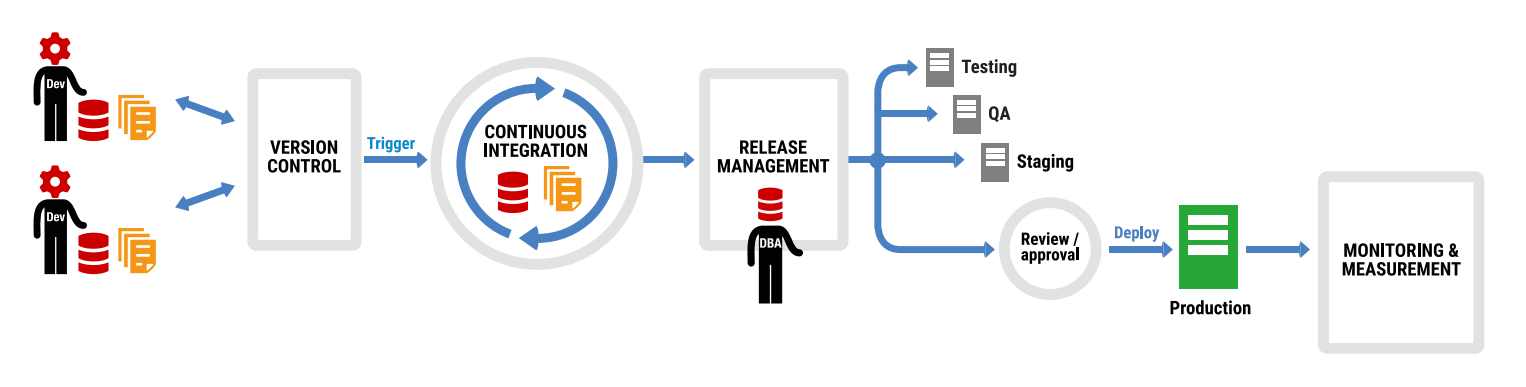
\includegraphics[width=14cm]{./IMAGENES/basededatos_1} 
		\caption{Incluyendo la base de datos en DevOps}
	\end{center}
\end{figure}

\subsubsection{\textbf{B2}}

EDITAR\\

%% TERCERA SUBSECCION
\subsection{\textbf{C}}

\subsubsection{\textbf{C1}}

EDITAR\\

\begin{itemize}

\item x
\item y
\item z

\end{itemize}
\subsubsection{\textbf{C2}}

EDITAR\\


%% ----------------------------------------------------------------------------------------------------------------------------------
 


%% ANÁLISIS ( APLICACIÓN ) ---------------------------------------------------------------------------------------------------

\section{Análisis}

\subsection{\textbf{Análisis 1}}
EDITAR\\

\subsection{\textbf{Análisis 2}}
EDITAR\\

\subsection{\textbf{Análisis 3}}
EDITAR\\

\subsection{\textbf{Análisis 4}}
EDITAR\\

%% ----------------------------------------------------------------------------------------------------------------------------------


%% CONCLUSIONES ---------------------------------------------------------------------------------------------------------------

\section{Conclusiones}

\begin{itemize}

\item Conclusion 1 : \\

\item Conclusion 2 : \\ 

\item Conclusion 3 : \\ 

\item Conclusion 4 : \\ 
\end{itemize}

%% ----------------------------------------------------------------------------------------------------------------------------------

%%  REFERENCIAS BIBLIOGRÁFICAS ------------------------------------------------------------------------------------------
	
	\newpage
	
	\bibliographystyle{apalike} 	%ESTILO
	\bibliography{BIBLIOGRAFIA}	 
	
	
\end{document}
